This project contains 4 big block components:
\begin{itemize}
 
\item Controller 

\item Google Cloud Speech API

\item OctoPrint

\item 3D Printer

\end{itemize}

Function of each component:

\begin{itemize}

\item Controller: Takes speech and .STL file as input.

\item Google Cloud Speech API: receives speech from user, then converts speech to text. 

In the other words, Google Cloud Speech API works as a audio transcription.

\item OctoPrint: interface to adjust setting on the printer and to print object.

\item 3D Printer: print 3D object from user's commands.

\end{itemize}

\begin{figure}[h!]
	\centering
   	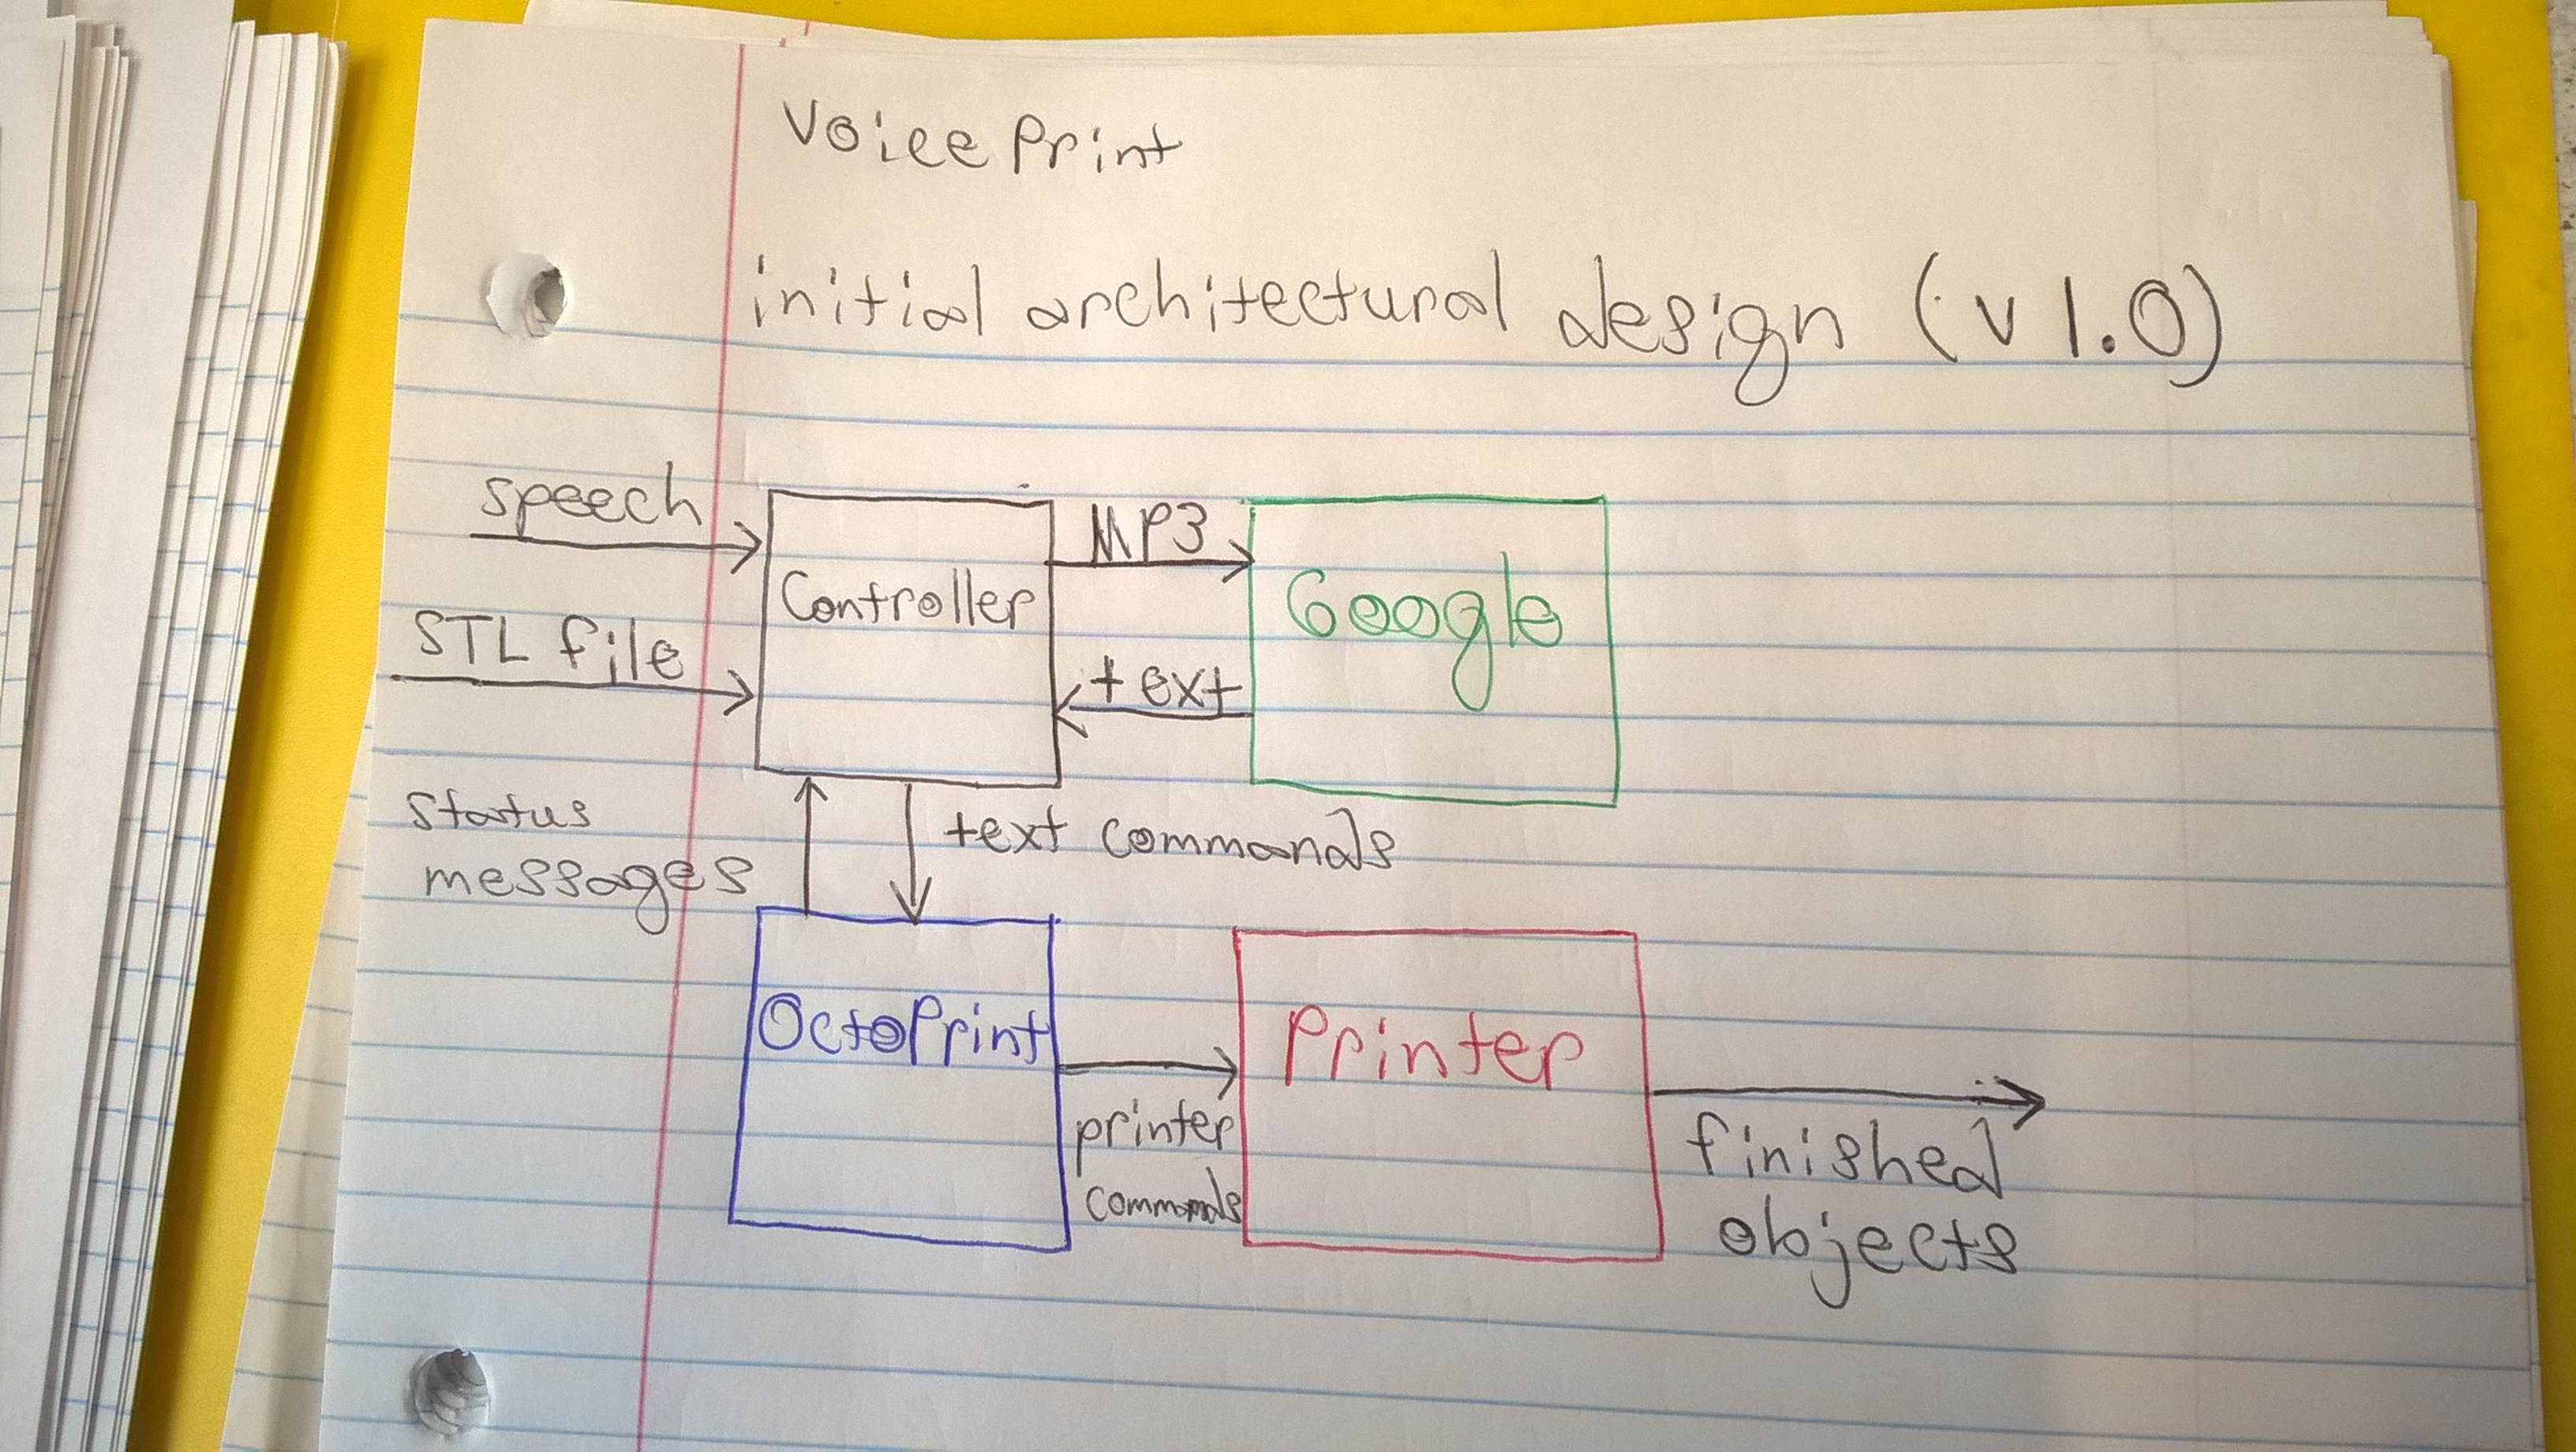
\includegraphics[width=0.6\textwidth]{images/Diagram.jpg}
   	    \caption{Diagram of major components of VoicePrint}

\end{figure}


